\begin{appendix}

\chapter{Sprints}

\chapter{Minutes}

\chapter{Time Logging}

%Simply export

\DTLloaddb{overview}{data/timelog-overview.csv}
\begin{table}[htbp]
  \caption{Overview By Member and Month}
  \centering
  \DTLdisplaydb{overview}
\end{table}

\begin{landscape}

\DTLsetseparator{,}
% don't forget to escape special characters like _ or # in the input .csv

\DTLloaddb{issueMember}{data/timelog-issue-member.csv}
  \centering
 \DTLdisplaylongdb[caption="Overview By Member and Issue"]{issueMember}

\DTLloaddb{sprints}{data/timelog-sprints.csv}
\begin{table}[htbp]
  \caption{Overview By Sprints}
  \centering
  \DTLdisplaydb{sprints}
\end{table}

\end{landscape}

\chapter{Mockups}

\section{Hand-Drawn}

\begin{figure}[!h]
  \centering
    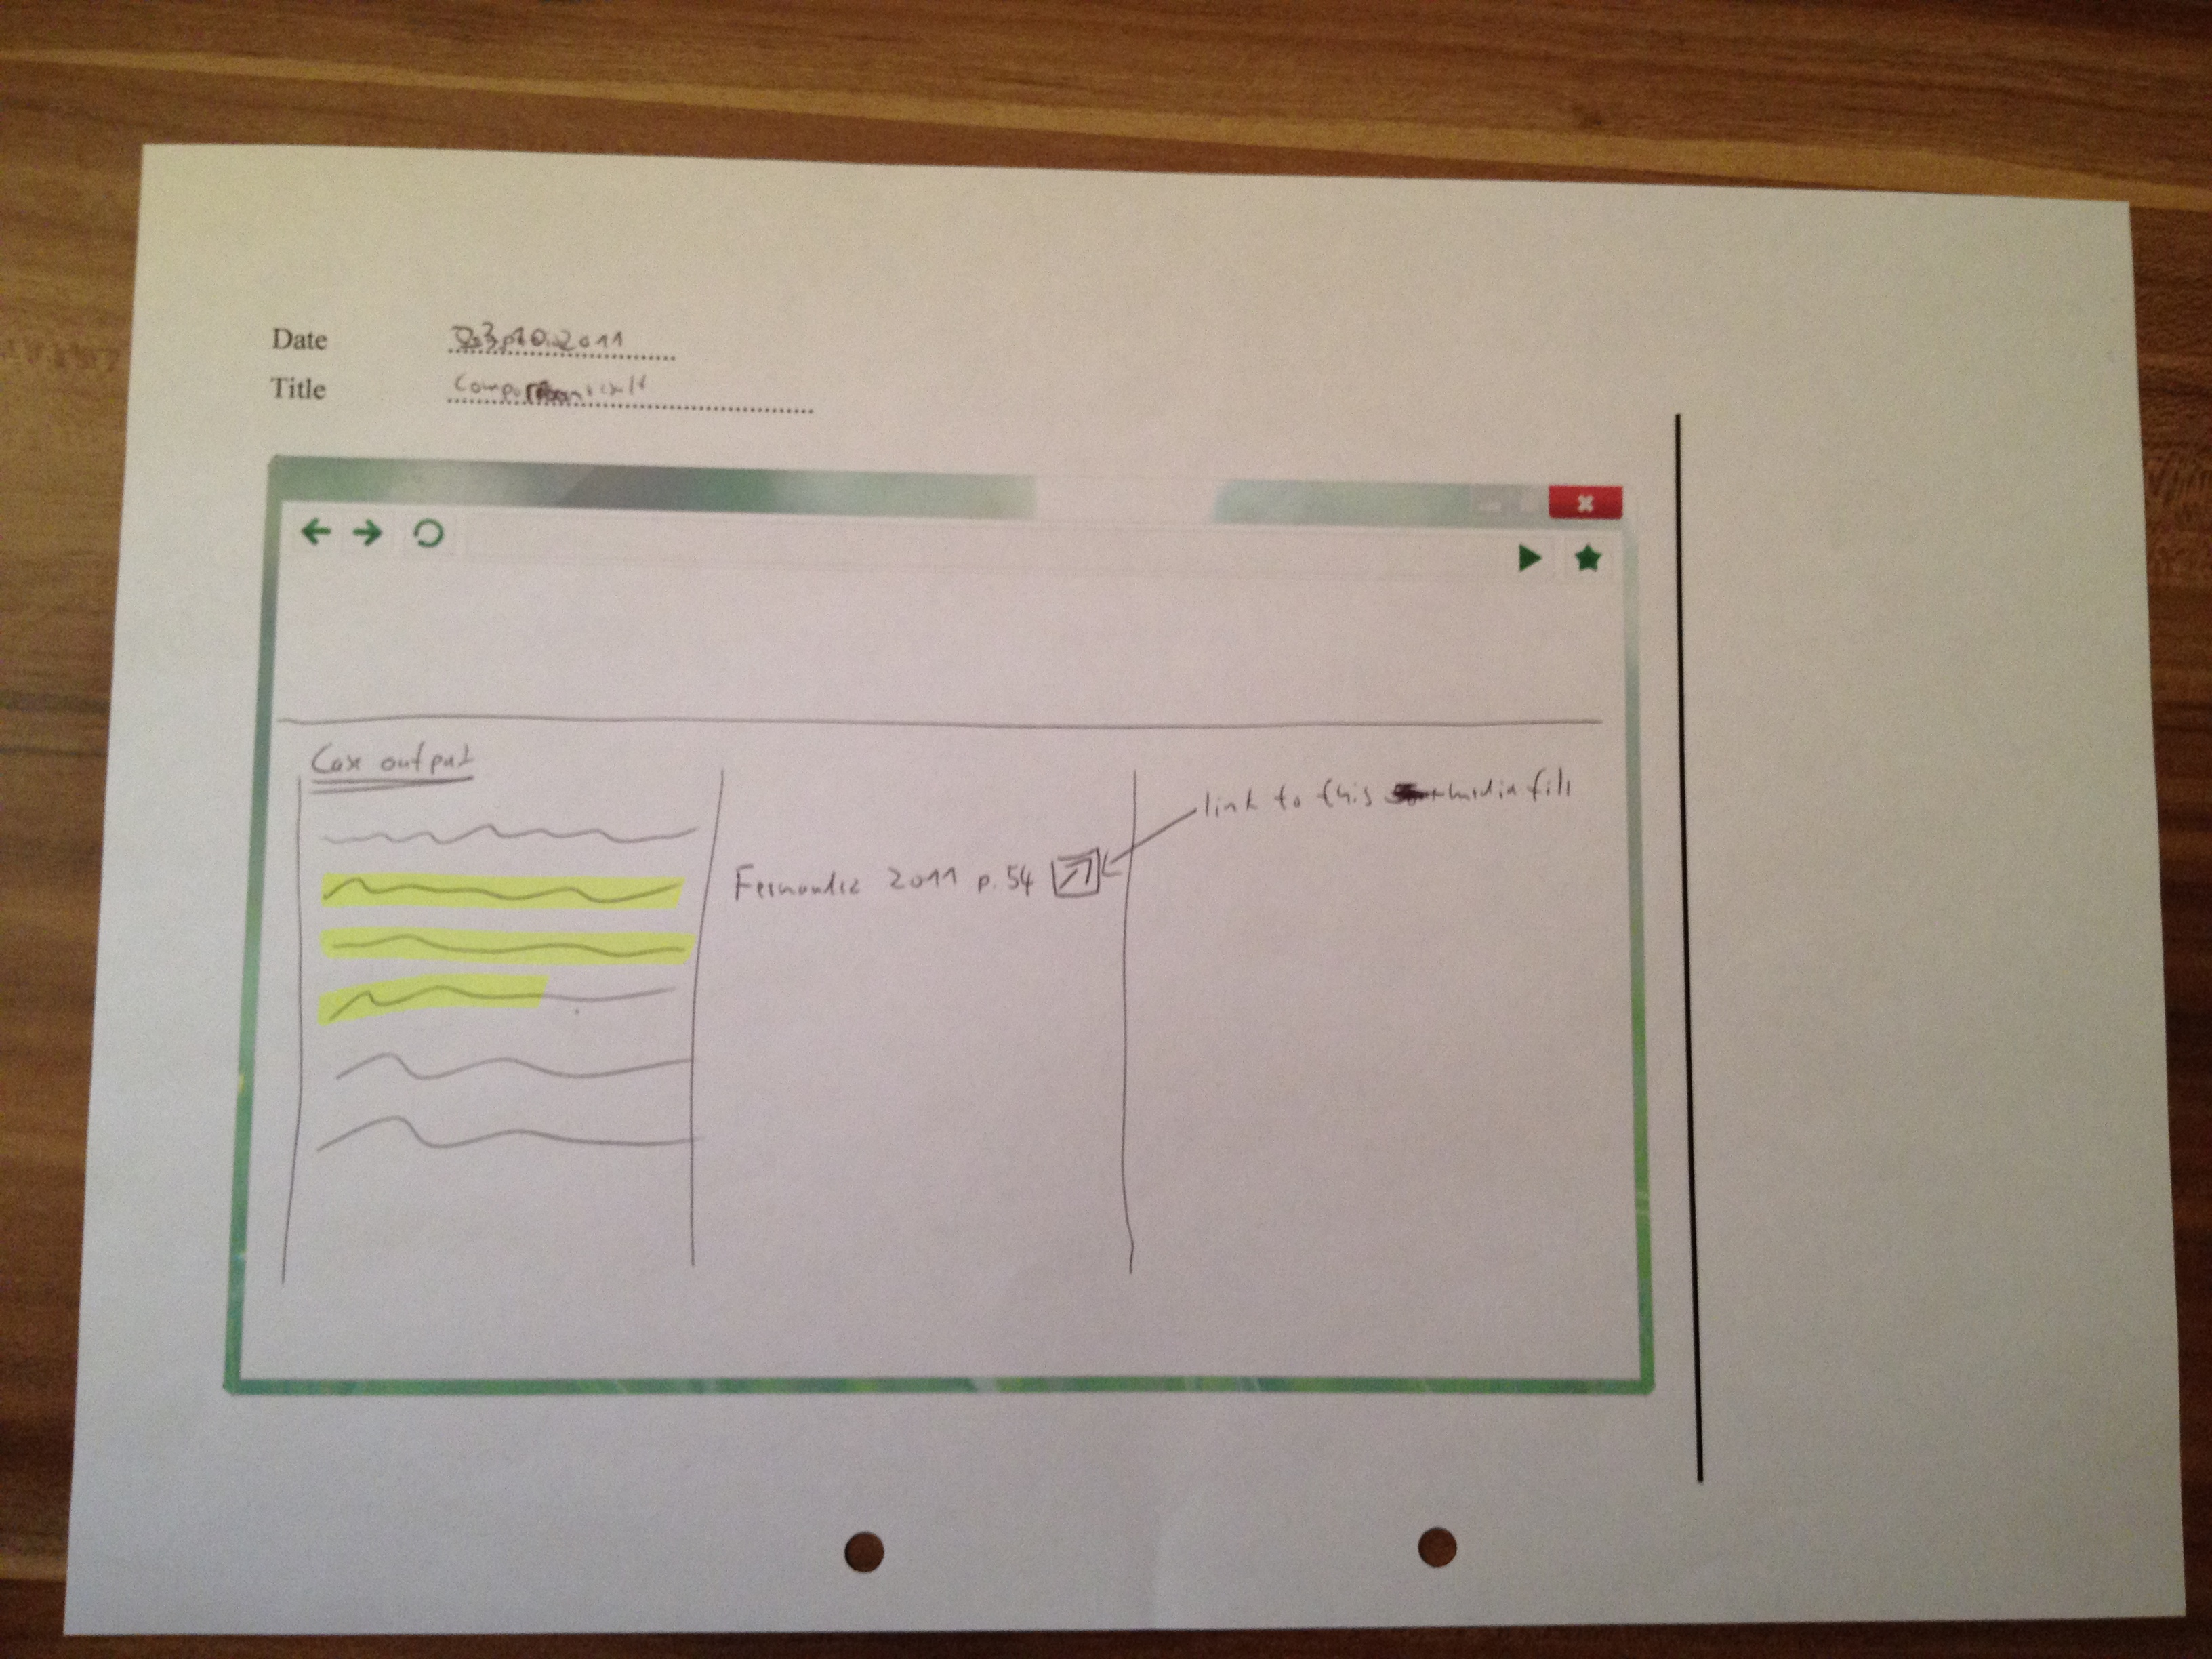
\includegraphics[width=\textwidth]{mockups/m_compare_result.jpg}
  \caption{Mockup – Compare results – digitalized }
  \label{fig:mCompareResultsMockup}
\end{figure}

\begin{figure}[!h]
  \centering
    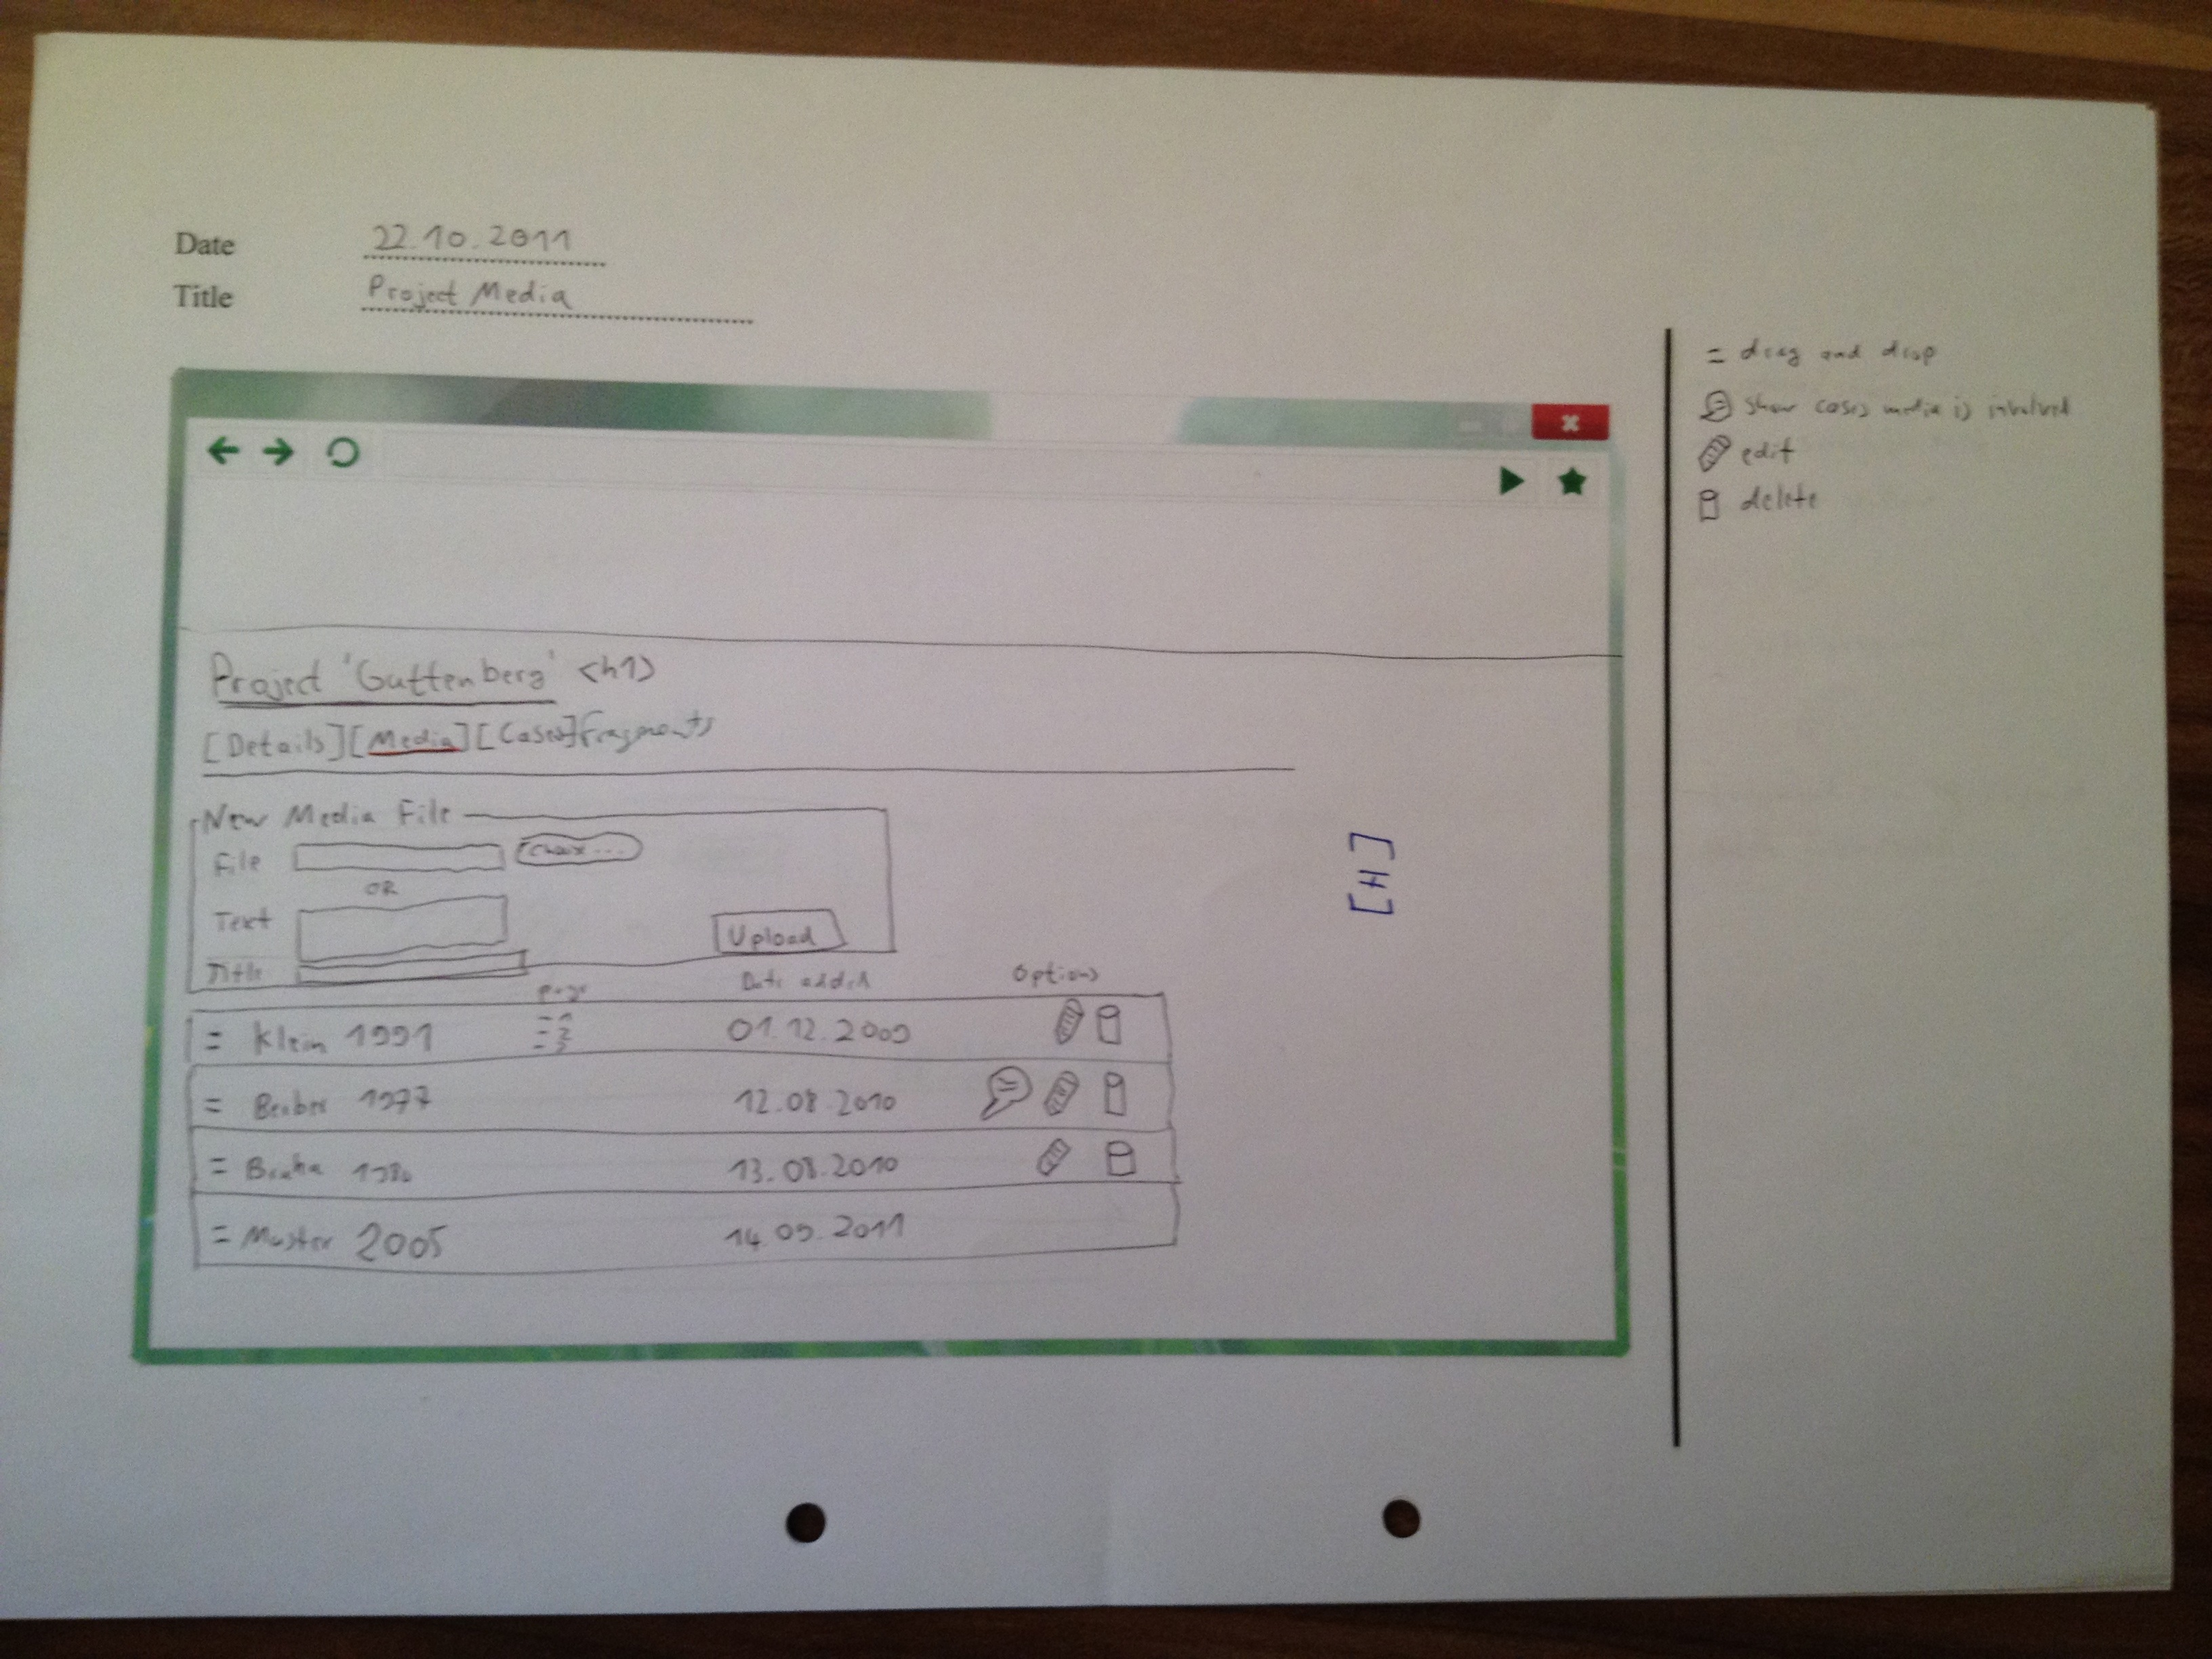
\includegraphics[width=\textwidth]{mockups/m_media_list.jpg}
  \caption{Mockup – Media list – digitalized }
  \label{fig:mMediaListMockup}
\end{figure}

\begin{figure}[!h]
  \centering
    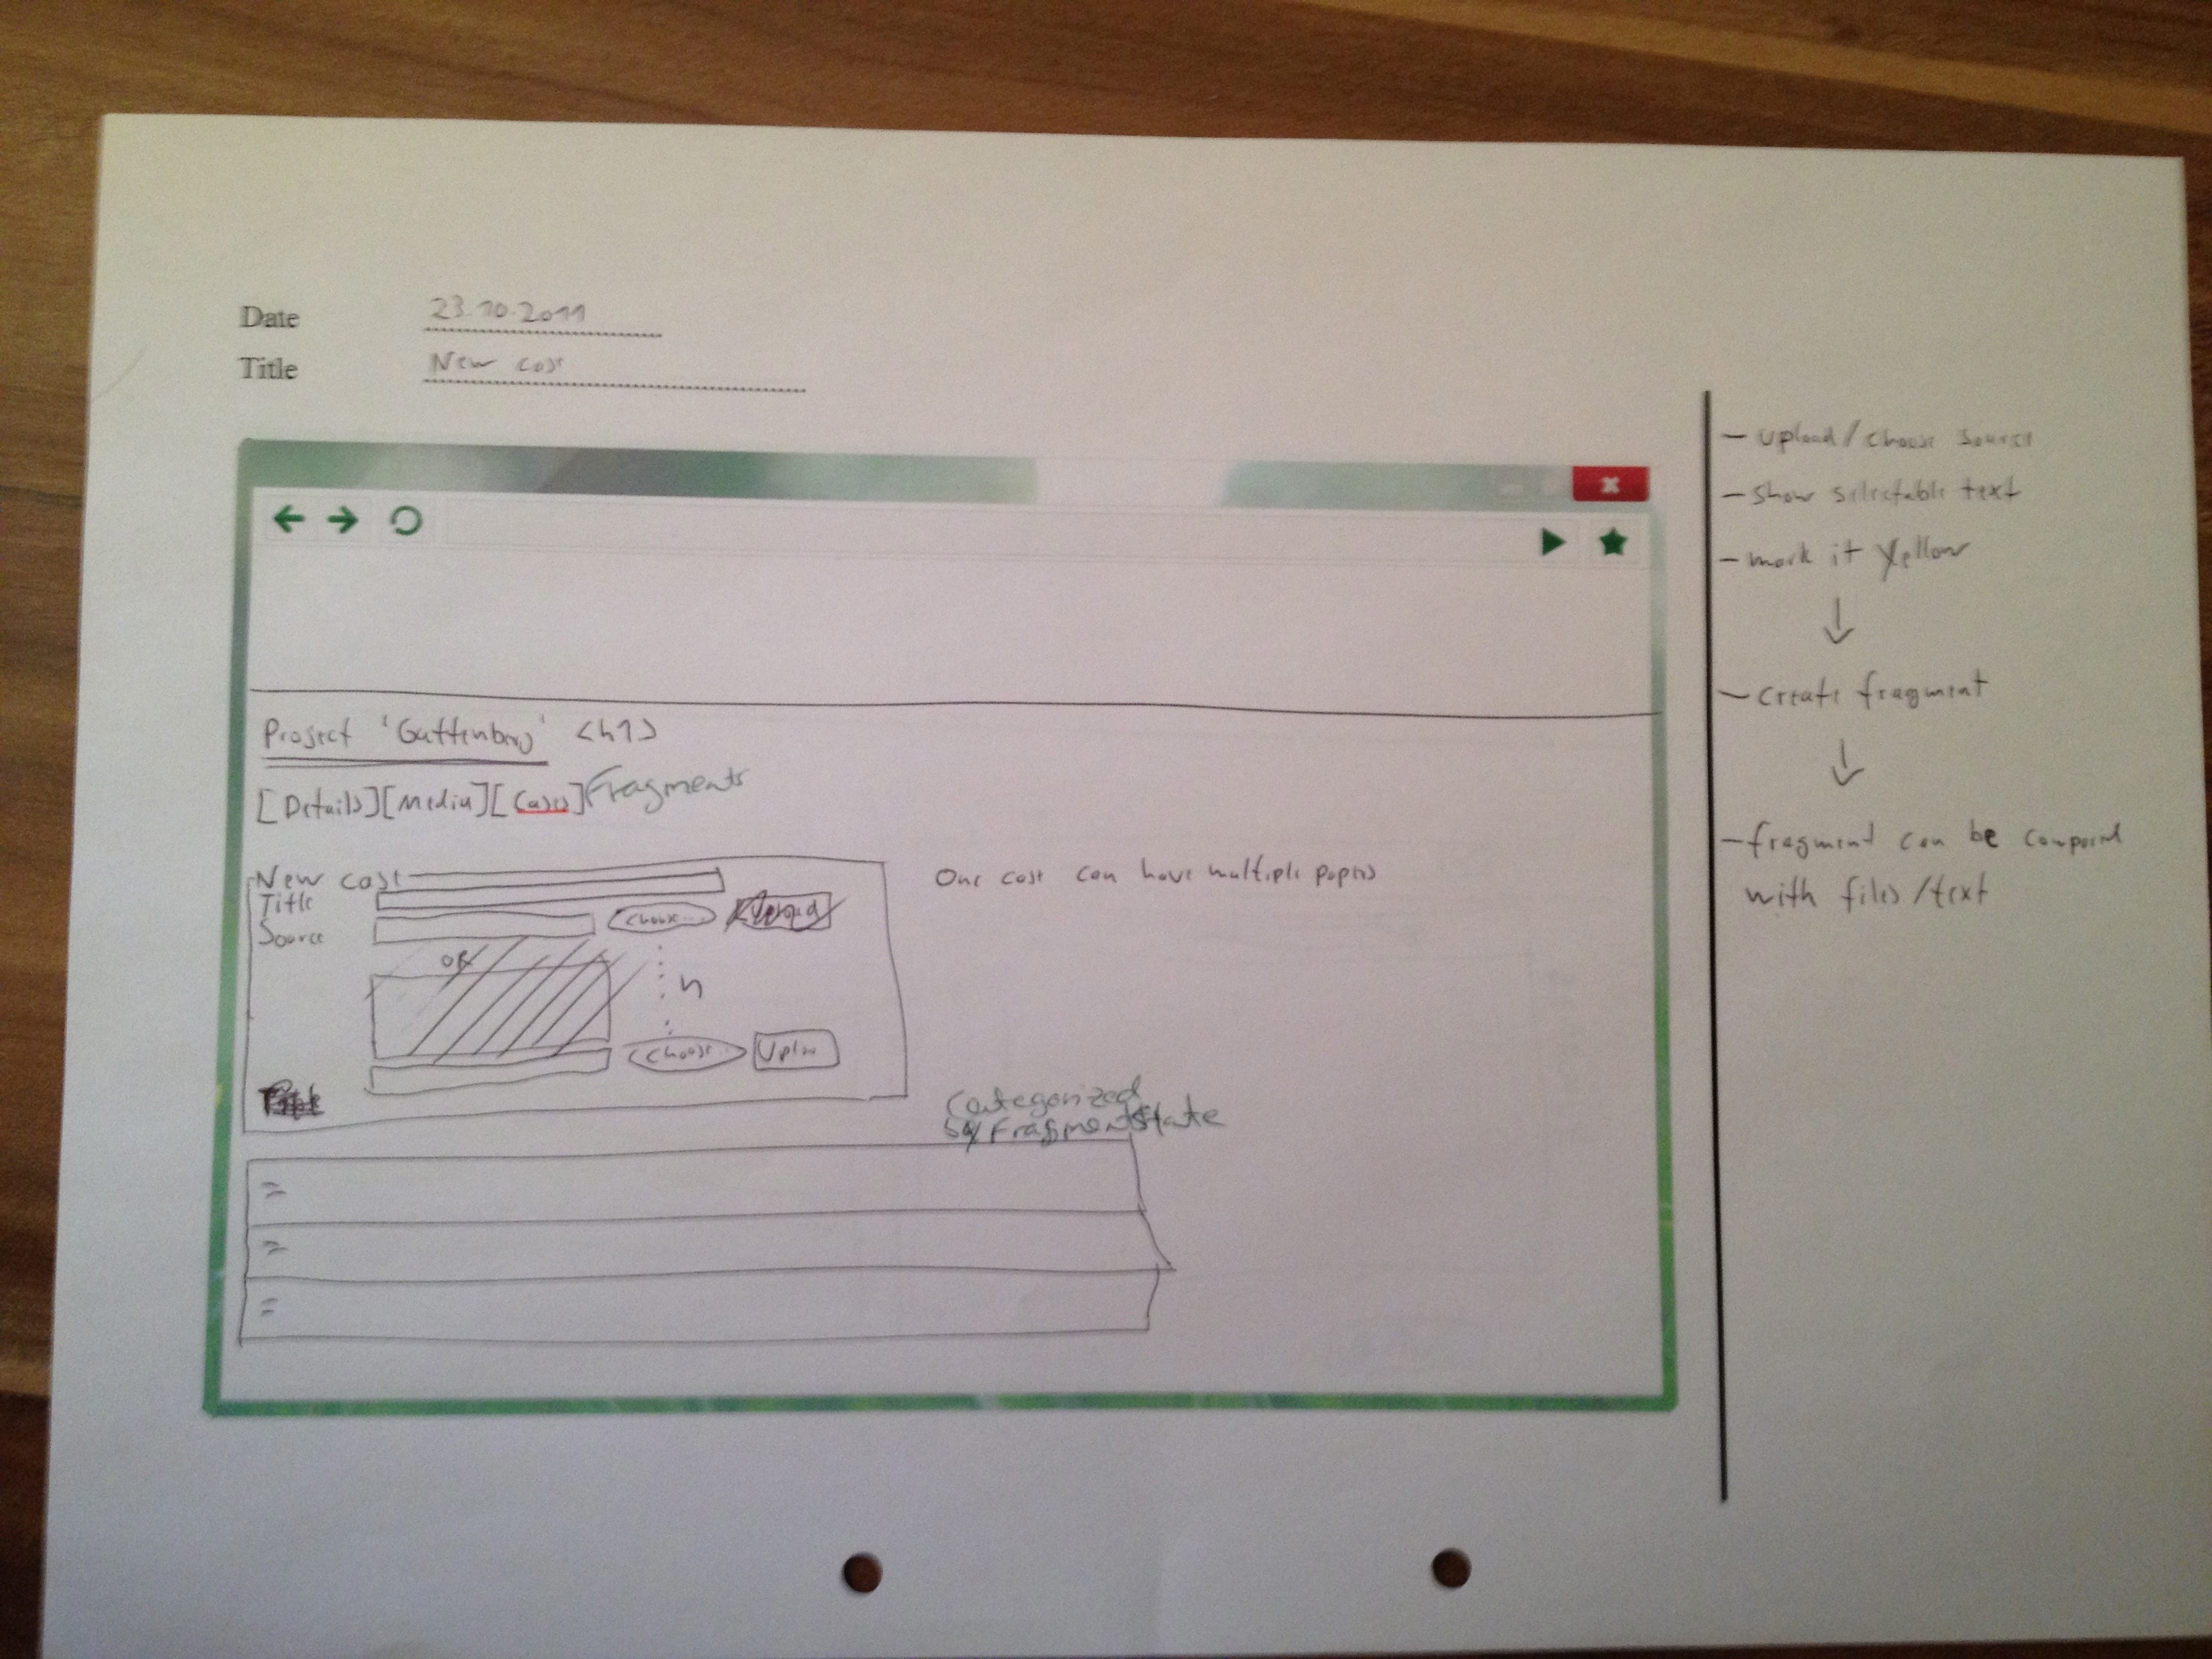
\includegraphics[width=\textwidth]{mockups/m_new_case.jpg}
  \caption{Mockup – New case – digitalized }
  \label{fig:1newCaseMockup}
\end{figure}

\begin{figure}[!h]
  \centering
    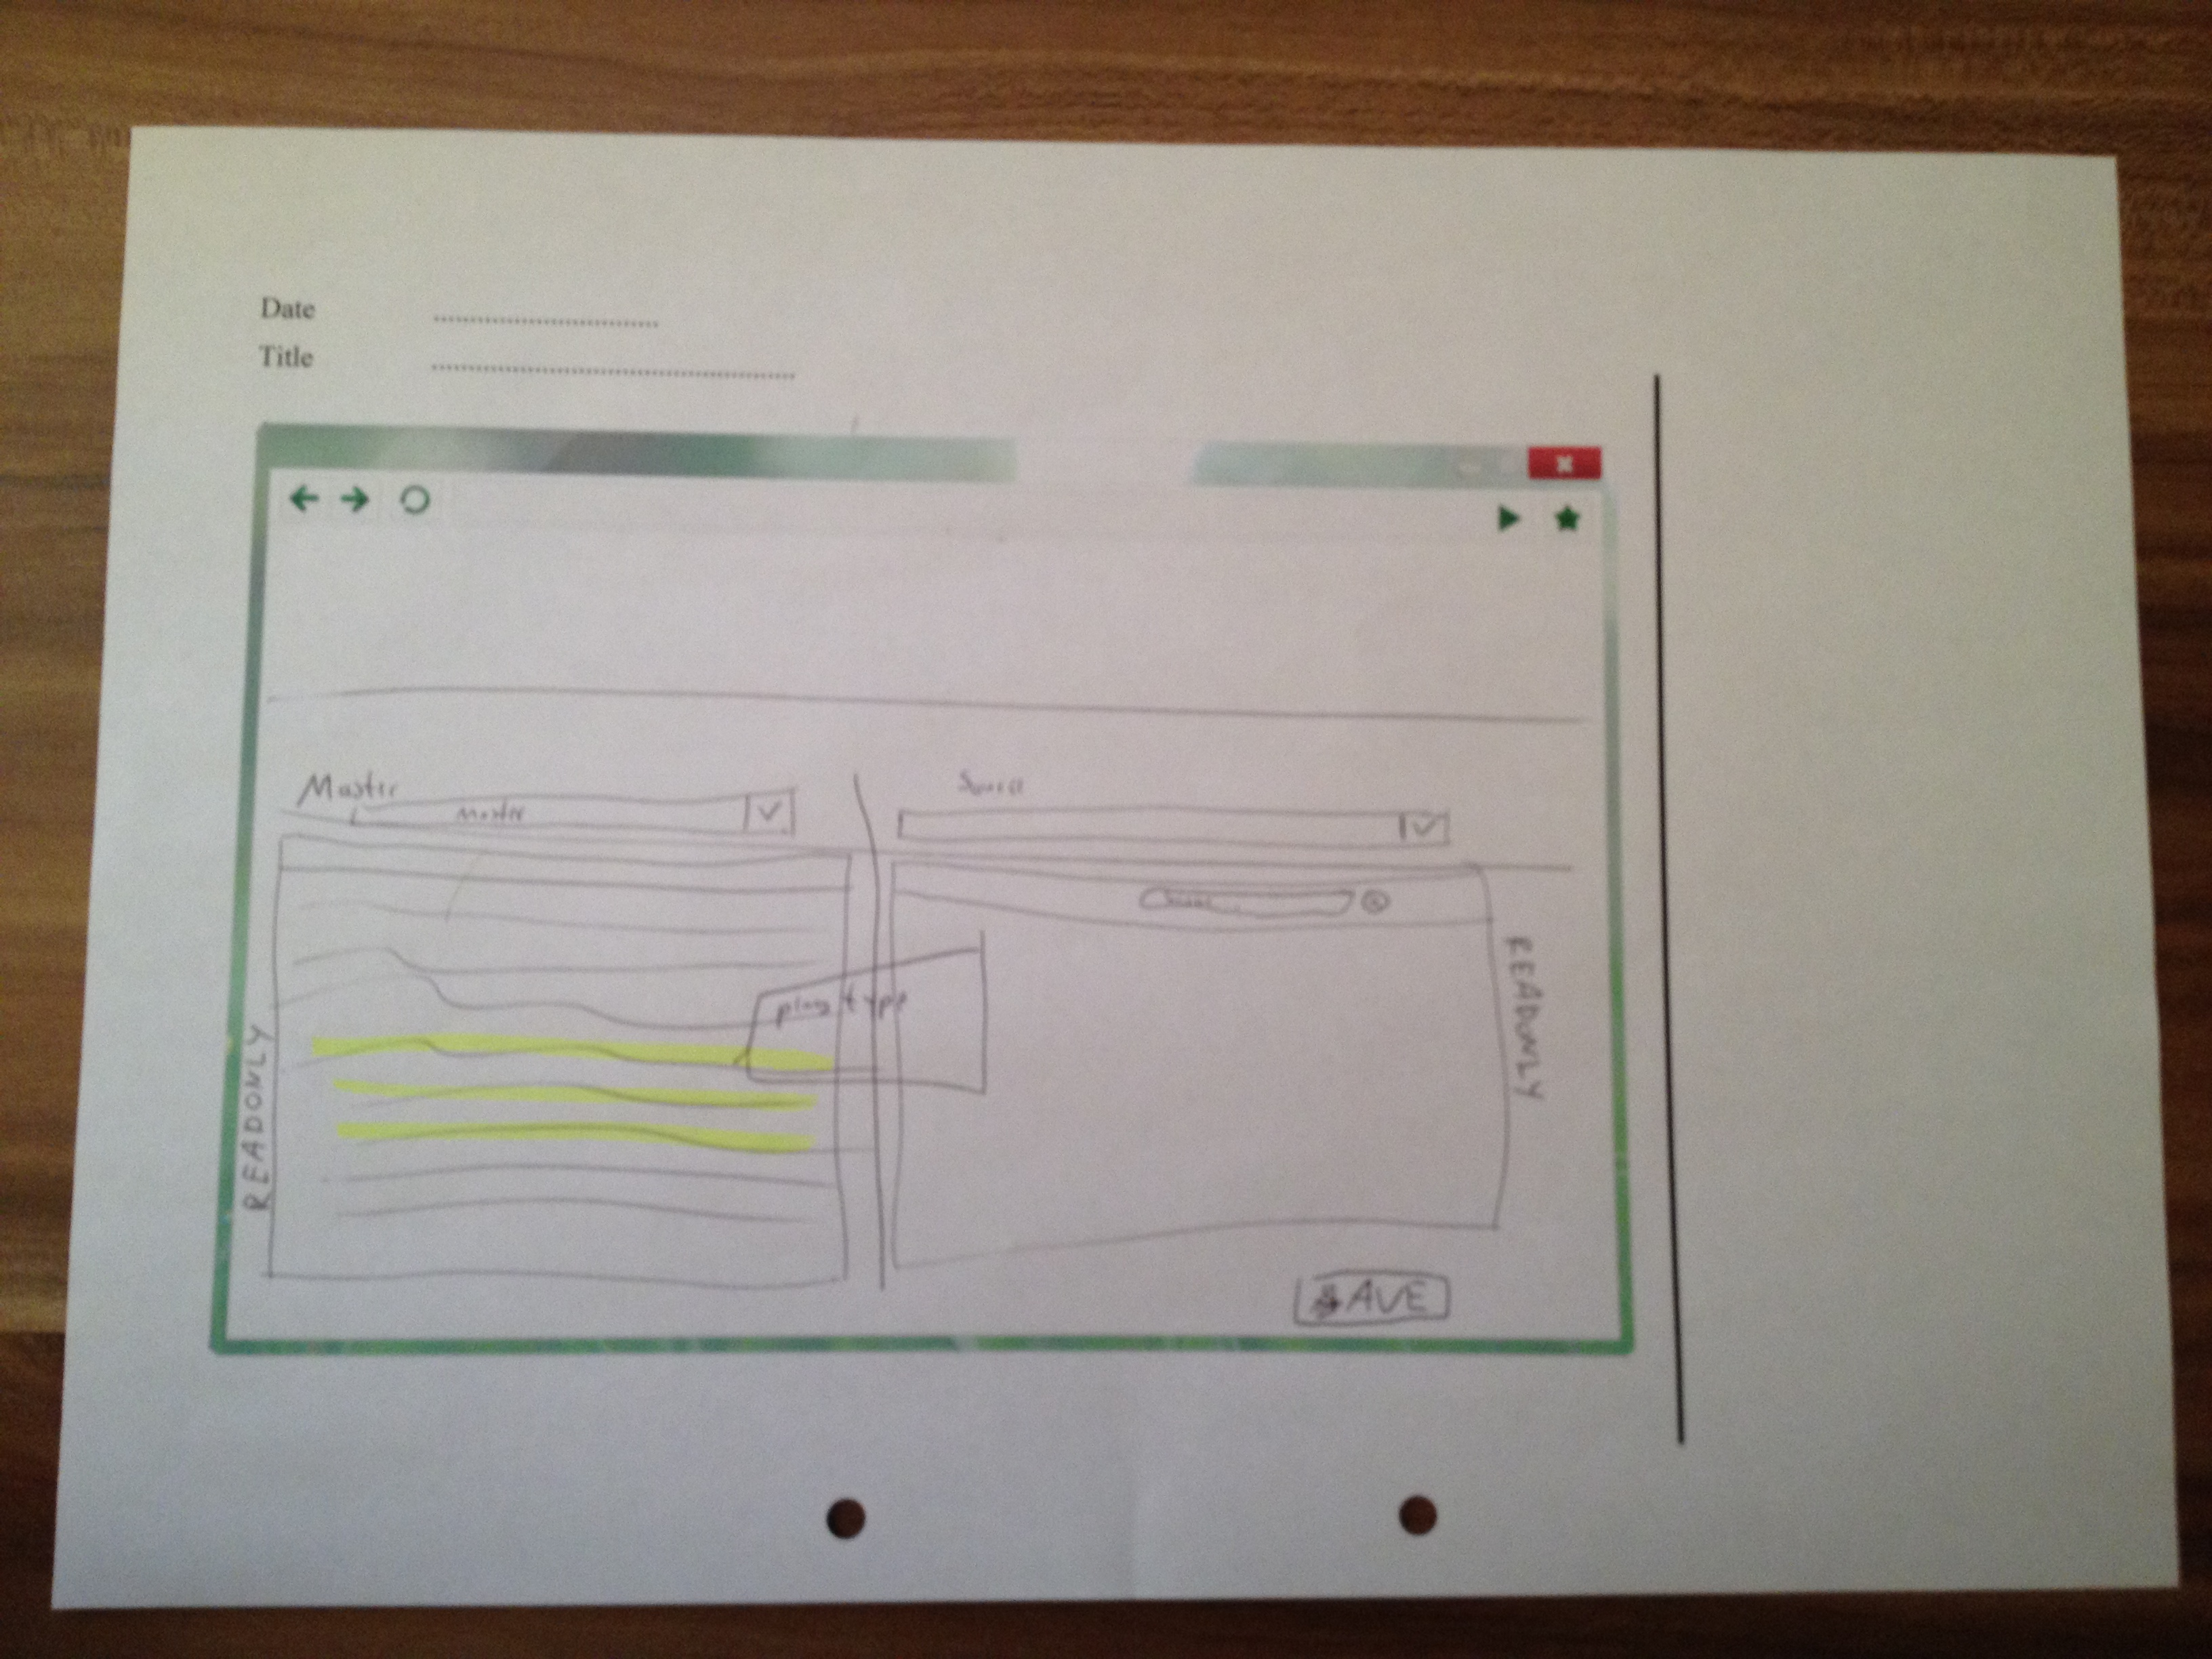
\includegraphics[width=\textwidth]{mockups/m_new_fragment.jpg}
  \caption{Mockup – New fragment – digitalized }
  \label{fig:1newCaseMockup}
\end{figure}

\begin{figure}[!h]
  \centering
    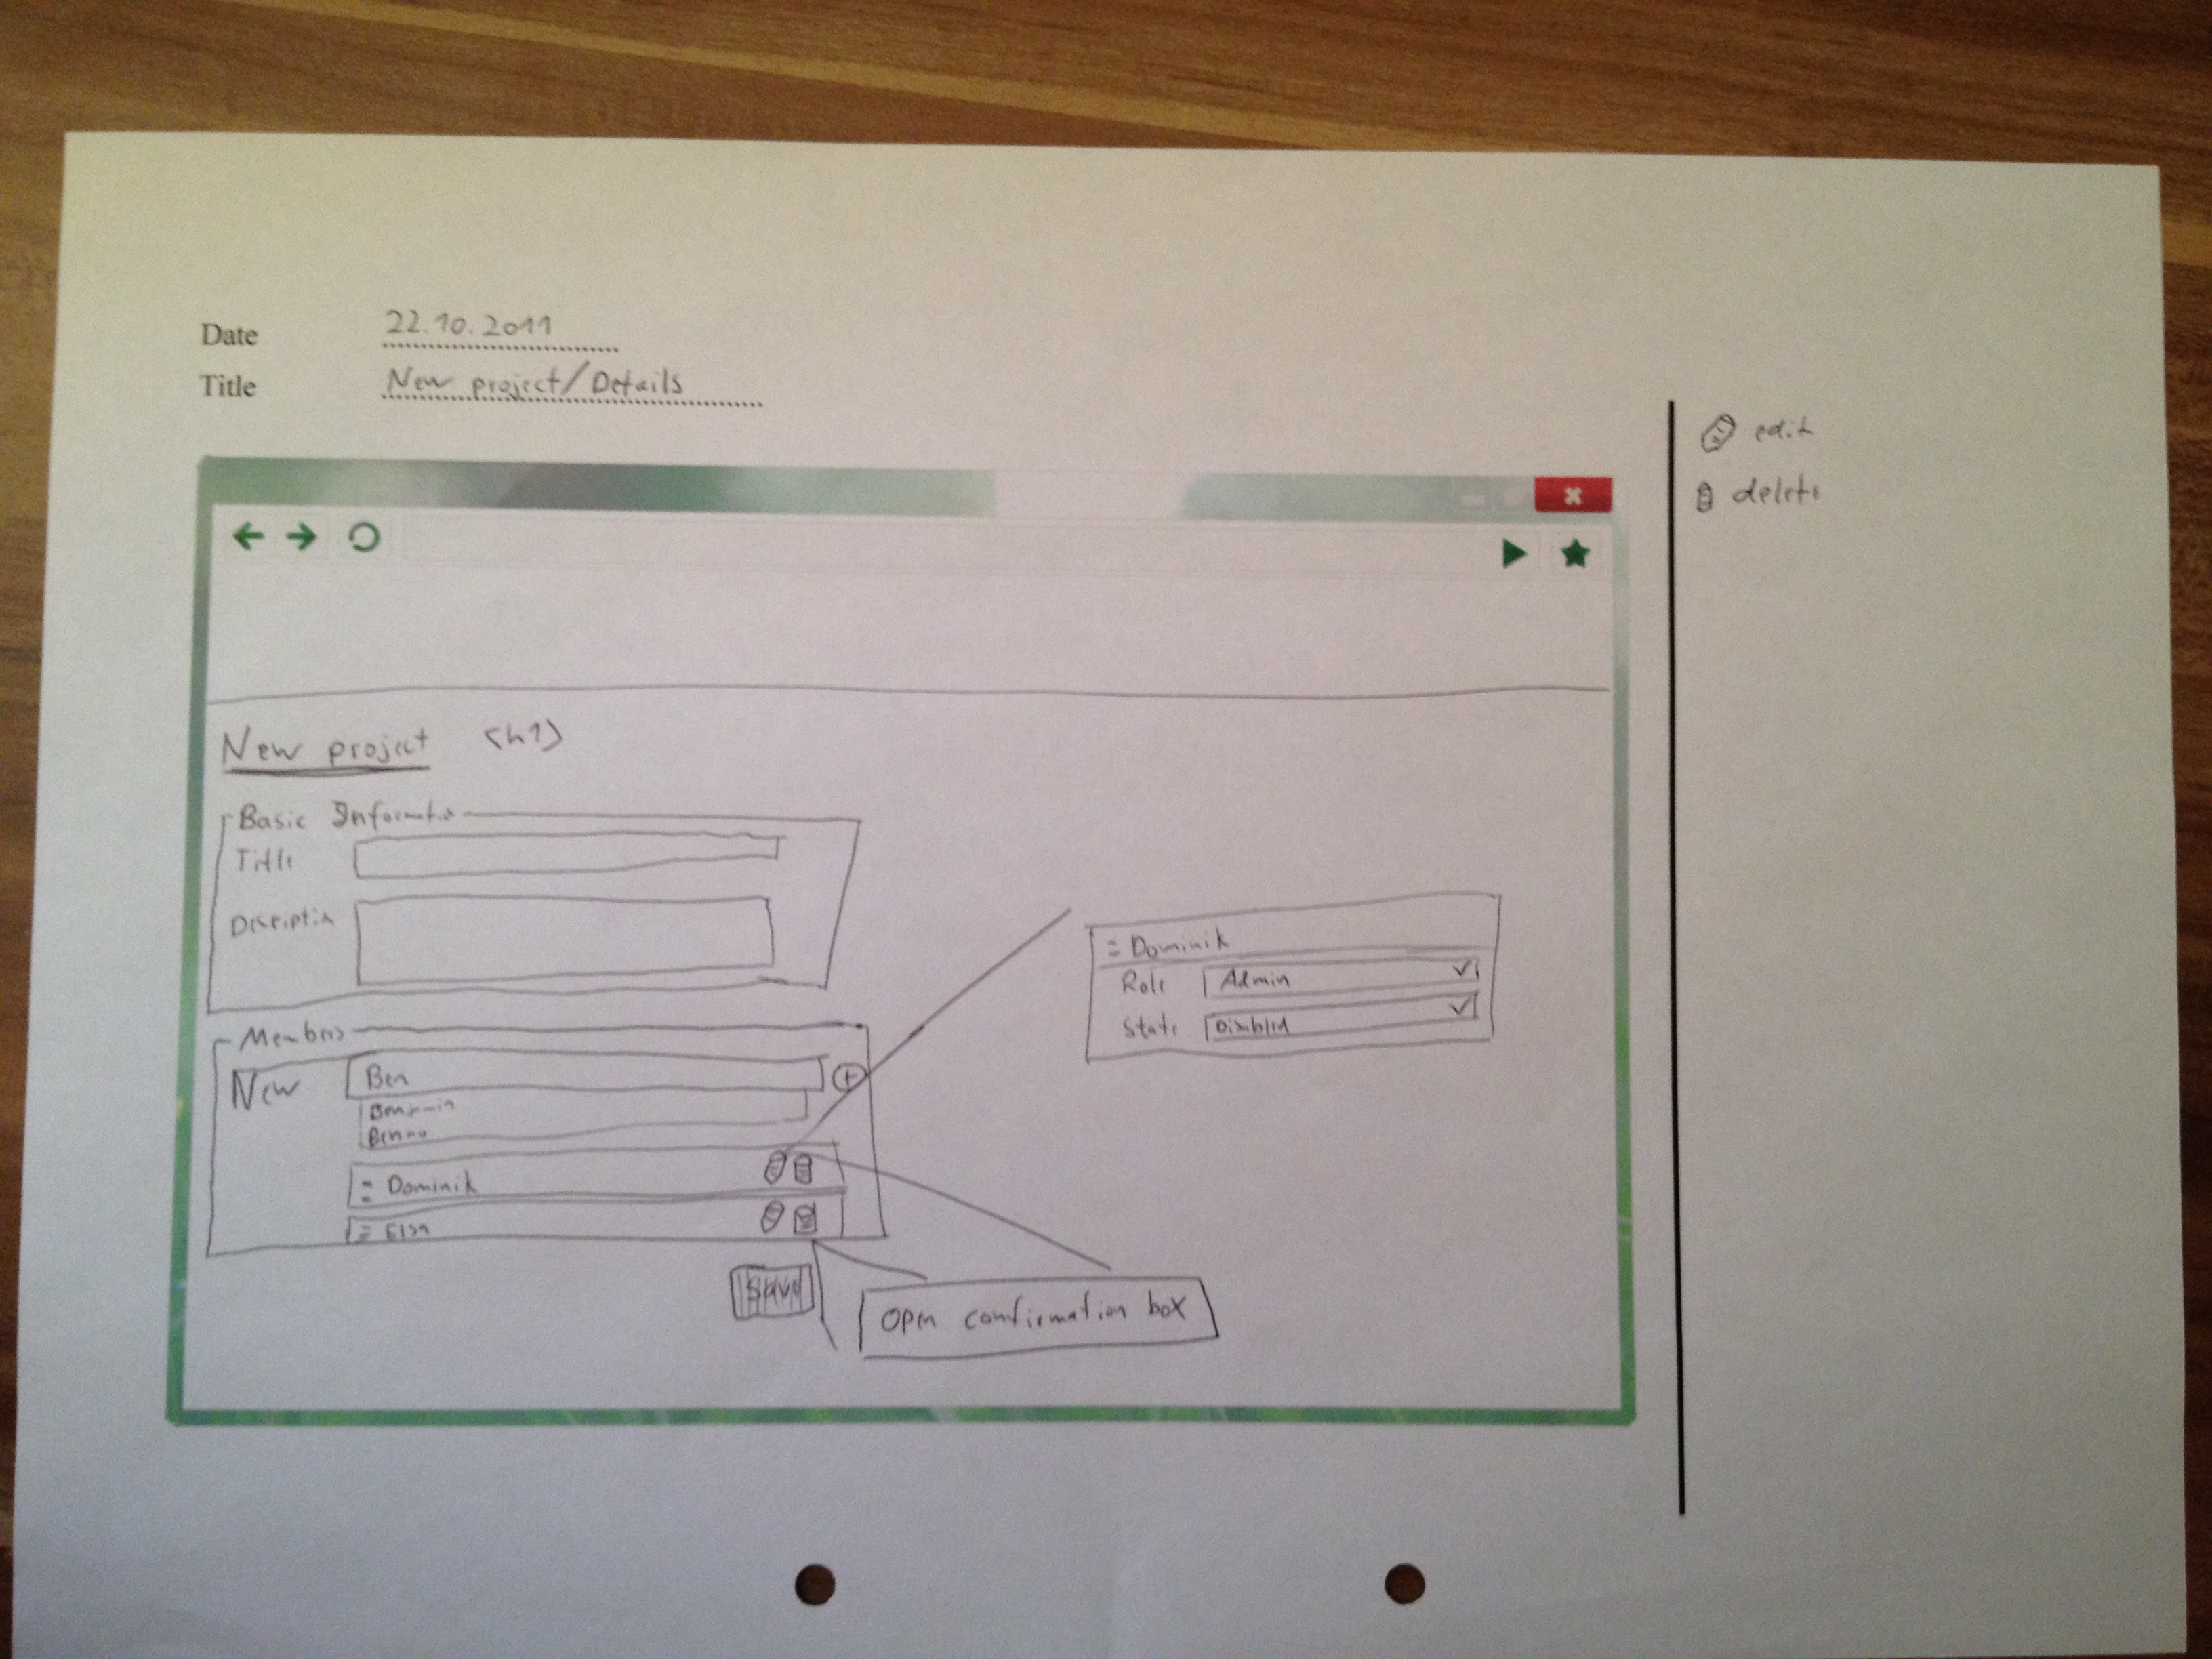
\includegraphics[width=\textwidth]{mockups/m_new_project.jpg}
  \caption{Mockup – New project – digitalized }
  \label{fig:mNewProjectMockup}
\end{figure}

\clearpage
\section{Digitalized}

\begin{figure}[htbp]
  \centering
    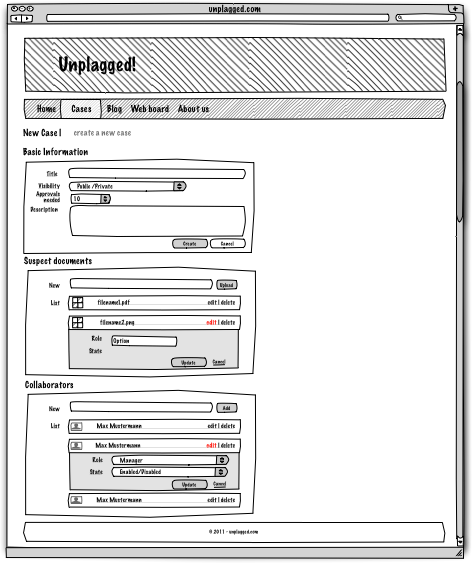
\includegraphics[width=0.86\textwidth]{mockups/1_new_case.png}
  \caption{Mockup – New case – digitalized }
  \label{fig:1newCaseMockup}
\end{figure}

\begin{figure}[!h]
  \centering
    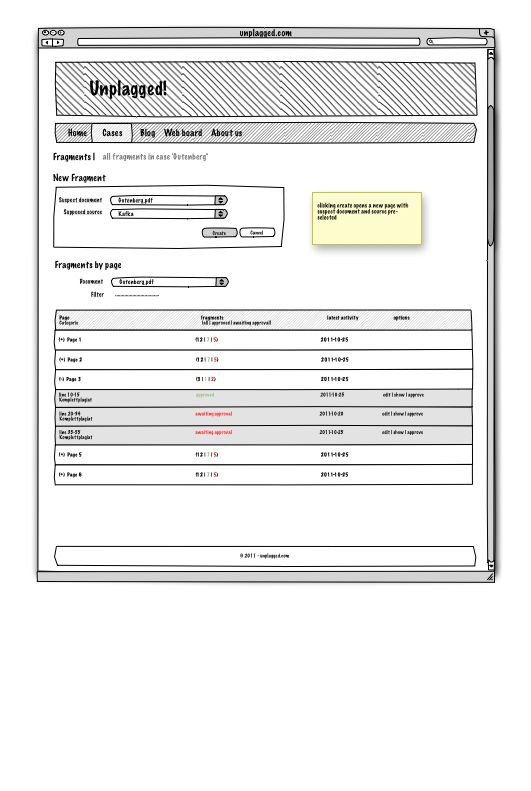
\includegraphics[width=\textwidth]{mockups/2_list_fragments.png}
  \caption{Mockup – List fragments – digitalized }
  \label{fig:2listFragmentsMockup}
\end{figure}

\begin{figure}[!h]
  \centering
    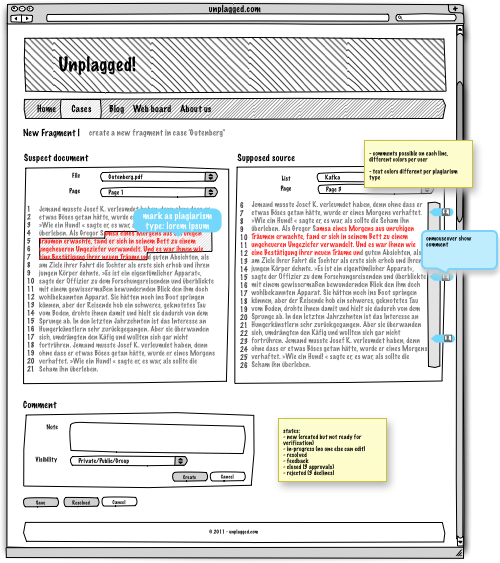
\includegraphics[width=\textwidth]{mockups/3_new_fragment.png}
  \caption{Mockup – New fragment – digitalized }
  \label{fig:3newFragmentMockup}
\end{figure}

\begin{figure}[!h]
  \centering
    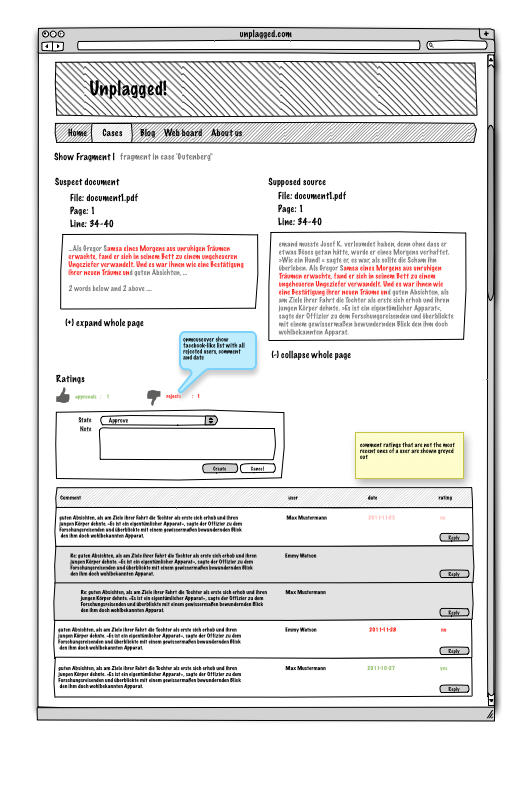
\includegraphics[width=0.97\textwidth]{mockups/4_show_fragment_for_approval.png}
  \caption{Mockup – Show fragment for approval – digitalized }
  \label{fig:4showFragmentForApprovalMockup}
\end{figure}

\begin{figure}[!h]
  \centering
    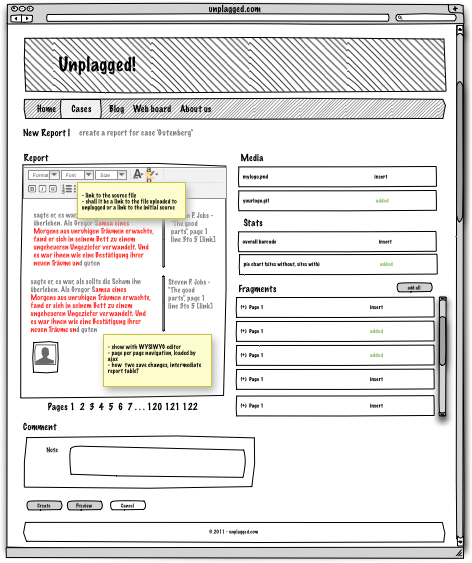
\includegraphics[width=\textwidth]{mockups/5_new_report.png}
  \caption{Mockup – New report – digitalized }
  \label{fig:5newReportMockup}
\end{figure}



\end{appendix}
